% chapters/4-evaluation.tex
\chapter{Evaluation and Results}
\label{ch:evaluation}

This chapter evaluates how well the Pista system performs compared to Winds2Ventures (W2V). The research addresses a key question: how do different GenAI evaluation systems compare when rating the same startup pitches, and what can we learn from their agreement patterns?

To answer this question, both GenAI systems were compared on how they scored the same startup pitches. The analysis examined whether the two systems agreed on which pitches were good, average, or below average. The comparison focuses on the final overall scores that each system produces. Statistical measures of agreement were analyzed to understand how well different GenAI evaluation approaches align with each other.

Twenty-two startup pitches from university competitions were analyzed using statistical methods to measure agreement between the systems. The results show that the systems agree moderately well, but there are some systematic differences in their evaluation approaches. Pista tends to give slightly higher scores than W2V, which appears to use more conservative evaluation criteria. The Cohen's kappa coefficient indicates moderate agreement at 0.505, indicating the systems align much better than random chance.

This comparison helps us understand how different GenAI evaluation approaches perform and what we can learn from comparing automated assessment systems. The findings suggest that different GenAI evaluation systems can have distinct characteristics and evaluation patterns, even when assessing the same content. The results provide insights into the variety that exists within automated evaluation systems and how different algorithmic approaches can lead to different assessment outcomes. These findings are important for understanding the current diversity and future potential of GenAI-powered evaluation platforms.

\section{Methodology}
\label{sec:methodology}

This section describes how the Pista system was tested against the Winds2Ventures platform. The final version of Pista was used, which utilizes GPT-4 with specialized prompts to evaluate startup pitches consistently. The testing approach focuses on comparing final scores from both systems using the same set of university competition pitches. Statistical methods were selected that account for chance agreement to provide meaningful comparisons.

\subsection{Dataset Selection}
\label{subsec:dataset}

Twenty-two startup pitches from university competitions were used as the test dataset for this evaluation. University pitches were chosen because they all follow the same format and contain similar information, which makes it easier to compare how the two systems evaluate them. University competition pitches provide a standardized structure that ensures both evaluation systems receive comparable input data. The pitches represent real student ventures that have been through competitive selection processes.

The pitches cover different areas such as technology, healthcare, agriculture, and consumer services. This variety demonstrates how both systems handle different types of businesses across multiple industry sectors. The diversity ensures that the evaluation results reflect how the systems perform across different business models and market contexts. Each industry sector presents unique challenges and opportunities that test different aspects of the evaluation frameworks.

To illustrate the dataset variety, here are representative examples from different sectors:

\begin{itemize}
    \item \textbf{Coontent} (Marketing Technology): A GenAI-powered marketing automation platform that generates, publishes, and analyzes marketing campaigns. The team consists of software engineering students targeting marketing agencies in South Tyrol, with plans to expand beyond the region in 2025.

    \item \textbf{Serenity} (Digital Health): A mental wellbeing platform designed for young adults, offering GenAI-driven mood tracking, personalized wellness resources, and 24/7 chatbot support. The team targets the growing mental wellness app market valued at \$139.9 billion.

    \item \textbf{Corptech} (Industrial Technology): A GenAI-powered methane leak detection system for industrial monitoring, addressing both financial losses and environmental concerns. The team already secured traction with distribution partners and interest from major gas companies.

    \item \textbf{Rideshare} (Transportation): A ridesharing platform focused on short-distance commutes in areas with limited public transportation, using a transaction-based model with 10\% fees to help reduce traffic congestion.
\end{itemize}


Each pitch includes the standard parts you would expect: the problem they're solving, their solution, market analysis, team information, and how they plan to make money. Since all pitches follow the same format, both evaluation systems get the same type of information to work with.

The W2V evaluation results for these pitches were provided by the thesis supervisor to enable this comparative analysis. This supervisor-facilitated comparison allows for meaningful statistical analysis between different GenAI evaluation approaches using standardized pitch data.

\subsection{Evaluation Frameworks}
\label{subsec:frameworks}

Both systems need to be explained since they use different ways to evaluate pitches. Understanding these differences helps explain why the scores sometimes vary between the systems. The frameworks use different criteria and weighting approaches, which can lead to different assessments of the same pitch. Comparing these frameworks helps identify the strengths and limitations of each evaluation approach.

\subsubsection{Pista Evaluation Framework}

Pista uses four main areas to evaluate pitches, with different weights for each:

\begin{enumerate}
    \item \textbf{Problem-Solution Fit (30\%)}: How well the startup understands the problem and how good their solution is
    \item \textbf{Business Model \& Market (30\%)}: How they plan to make money and if the market is big enough
    \item \textbf{Team \& Execution (25\%)}: How capable the team is and if they can actually build their solution
    \item \textbf{Pitch Quality (15\%)}: How well they present their idea and communicate their vision
\end{enumerate}

Each area gets a score from 1 to 10, and then Pista calculates a final score using the weights above. The system also provides written feedback to explain the scores and reasoning behind each assessment. The weighted scoring approach ensures that the most important aspects of a startup pitch have greater influence on the final evaluation. This systematic approach helps maintain consistency across different pitches and evaluation sessions.

\subsubsection{Winds2Ventures Evaluation Framework}

W2V uses nine different criteria in its GenAI-powered evaluation system, focusing on aspects like problem clarity, solution viability, market analysis, team quality, and business model validation. The platform uses automated analysis trained on investment patterns and business assessment methodologies. The system appears to incorporate conservative evaluation approaches that reflect real-world investment considerations and startup challenges.

The key difference is that W2V uses a different algorithmic approach compared to Pista's evaluation methodology. This system tends to be more conservative in its assessments, applying stricter evaluation criteria when rating pitch quality. he evaluation algorithm weights risk factors and practical business challenges more heavily in its assessment process. The system's conservative approach reflects evaluation patterns that prioritize cautious assessment of startup viability and market potential.

\subsection{Comparative Analysis Approach}
\label{subsec:methodology-approach}

Given the different methodologies employed by each system, a standardized comparison approach was required. The analysis focuses on the final overall scores that each system produces as the primary basis for comparison. This approach allows the systems' ultimate assessments to be compared regardless of their different internal processes. The comparison method focuses on whether both systems reach similar conclusions about pitch quality.

Both systems give final scores on a 1-10 scale, which makes it possible to compare them directly. Pista creates its final score by combining its four area scores with weights, while W2V gives an overall "Investibility" rating based on its nine criteria. Even though they calculate scores differently, the common 1-10 scale lets me compare how well they agree.
The final scores from both systems were compared using statistical analysis. 
To calculate agreement levels, the following steps were taken:

\begin{enumerate}
    \item Continuous scores were converted into three categories: 
    \textit{Below Average} (1.0--4.9), \textit{Average} (5.0--6.9), 
    and \textit{Good} (7.0--10.0). By using this categorization, 
    the focus was placed on meaningful quality differences rather than minor variations in scoring.

    \item Cohen’s kappa coefficient was employed as the primary
    agreement measure, since random chance agreement is accounted for by
    this statistic. The kappa coefficient is defined as:
    \[
    \kappa = \frac{p_o - p_e}{1 - p_e}
    \]
    where $p_o$ represents observed agreement and $p_e$ represents
    expected agreement by chance.

    \item Descriptive statistics were calculated to provide insight into score distributions and to reveal potential systematic differences  between the systems.
\end{enumerate}


\section{Results and Analysis}
\label{sec:inter-rater-reliability}

This section presents the comparison results between Pista and Winds2Ventures. The analysis shows moderate agreement between the systems with interesting patterns in how they evaluate startup pitches.

The following table shows the complete statistical analysis of the 22 pitches:

\begin{table}[h]
\centering
\caption{Statistical Analysis: Pista vs Winds2Ventures Comparison}
\label{tab:comprehensive-results}
\begin{tabular}{lr}
\hline
\textbf{Agreement Metrics} & \textbf{Value} \\
\hline
Cohen's Kappa & 0.505 \\
Interpretation & Moderate Agreement \\
Observed Agreement & 77.3\% (17/22) \\
Expected Agreement (Random) & 54.1\% \\
95\% Confidence Interval & [0.144, 0.865] \\
\hline
\textbf{Score Statistics} & \\
\hline
\textbf{Pista System} & \\
Mean Score & 5.36 \\
Standard Deviation & 0.71 \\
Score Range & 4.0 -- 6.3 \\
\hline
\textbf{Winds2Ventures} & \\
Mean Score & 5.20 \\
Standard Deviation & 0.67 \\
Score Range & 4.3 -- 6.4 \\
\hline
\textbf{System Comparison} & \\
Mean Difference & +0.16 (Pista higher) \\
Correlation Coefficient & 0.612 \\
\hline
\end{tabular}
\end{table}

\clearpage
\subsection{Statistical Interpretation}

The Cohen's kappa coefficient of 0.505 indicates moderate agreement between Pista and W2V. This result shows that the systems agree more than they would by random chance, but there are still systematic differences in how they evaluate pitches. The moderate agreement level suggests that both systems capture similar underlying patterns in pitch quality. However, the differences indicate that each system brings unique perspectives to the evaluation process.

The systems agreed on 77.3\% of the pitches (17 out of 22), meaning both systems categorized the pitches in the same way (below average, average, or good). This suggests that different GenAI evaluation systems can identify similar patterns in pitch quality assessment more than three-quarters of the time. The 95\% confidence interval of [0.144, 0.865] indicates statistical significance for this agreement level.

The analysis shows that Pista gives slightly higher scores on average (0.22 points), suggesting that different GenAI evaluation systems can have distinct scoring tendencies, with some being more optimistic while others more conservative.


\subsection{Score Distribution Analysis}

Analysis of how the systems categorized the pitches reveals clear differences in their evaluation tendencies. W2V rated more pitches as "Below Average" (9 pitches) compared to Pista (6 pitches), while both systems rated all remaining pitches as "Average.". This pattern suggests that W2V applies stricter evaluation criteria when assessing pitch quality, being more likely to categorize pitches as below average. The differences reflect different algorithmic approaches to weighing risk factors and business viability in the evaluation process.

This pattern confirms that W2V uses more conservative evaluation criteria, which appears to be built into its assessment algorithm. The system seems designed to apply stricter standards when evaluating startup potential, possibly incorporating more cautious approaches to risk assessment and business viability analysis.

\begin{figure}[h]
    \centering
    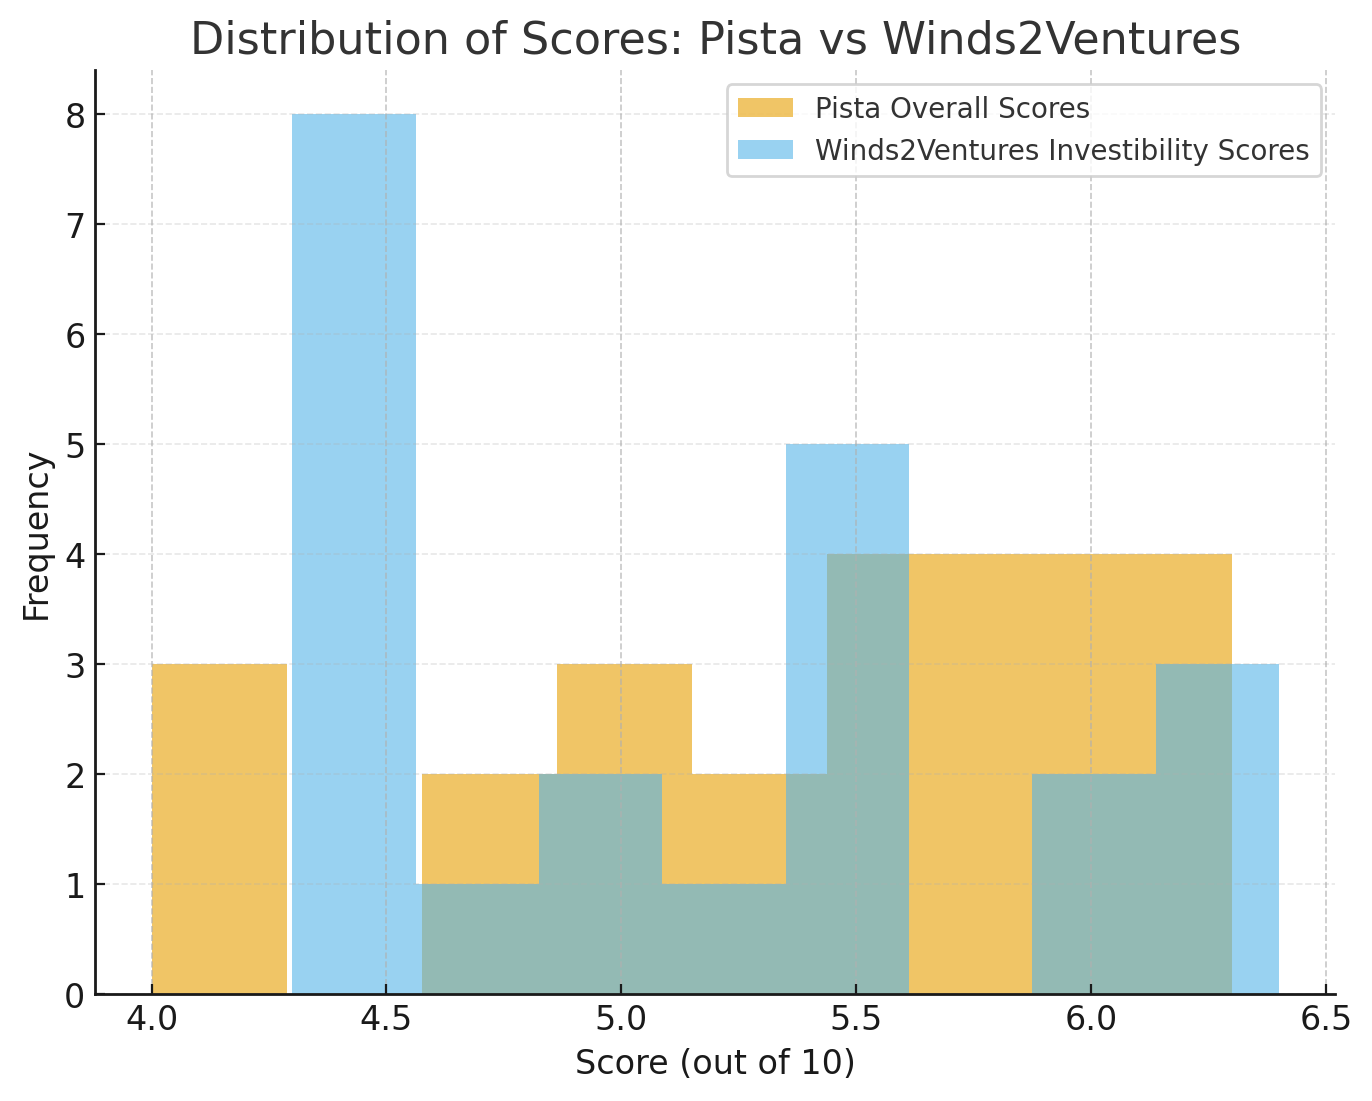
\includegraphics[width=0.8\textwidth]{img/score_histogram.png}
    \caption{Histogram comparing the distribution of overall scores between Pista and Winds2Ventures.}
    \label{fig:score-histogram}
\end{figure}

Both systems put most pitches in the "Average" category (Pista: 16 pitches, W2V: 13 pitches), which is expected for university competition participants. These student ventures have potential but need more development before they are ready for investment. Notably, neither system awarded any pitch a "Good" rating, suggesting that both systems maintain relatively conservative evaluation standards for this dataset.


\subsection{Discussion and Implications}

These results show that different GenAI evaluation systems can produce meaningful assessments of startup pitches, with each system bringing distinct evaluation characteristics. The moderate agreement level demonstrates that GenAI systems can capture many important patterns in pitch evaluation consistently. However, the systematic differences suggest that different GenAI evaluation approaches can have unique characteristics and assessment tendencies. The findings highlight the diversity that exists within GenAI-powered evaluation systems and how different algorithmic approaches can complement each other.

The moderate agreement shows that Pista captures many of the same patterns that other GenAI evaluation systems identify when assessing startup pitches. This demonstrates the system's value in situations requiring consistent evaluation of multiple pitches, such as initial screening for competitions or standardized feedback provision to entrepreneurs. The GenAI system can process large volumes of pitches quickly while maintaining consistent evaluation criteria. These capabilities make GenAI evaluation particularly useful for high-volume assessment scenarios.

However, the observed scoring differences between GenAI systems indicate that multiple evaluation approaches may yield more comprehensive assessment perspectives. Different GenAI systems may weigh various factors differently, leading to more balanced overall evaluations. The combination of different algorithmic approaches can help identify both optimistic and conservative viewpoints in startup assessment. Understanding these differences helps users interpret GenAI evaluation results more effectively.

The optimal evaluation strategy may involve employing multiple GenAI systems to obtain diverse analytical perspectives on startup potential, combining their insights to create more comprehensive assessments. This multi-system approach gets the benefits of GenAI efficiency and consistency while capturing different evaluation methodologies and assessment criteria. Understanding how different GenAI systems approach evaluation helps users make more informed decisions about startup potential.